\documentclass[UTF8,11pt,a4paper,fontset=windows]{ctexart}
\usepackage[margin=24mm,headheight=15pt]{geometry}
\usepackage{amsmath,amssymb,mathtools,graphicx,booktabs,enumitem,needspace,fancyhdr,xcolor,hyperref}
\hypersetup{unicode=true,hypertexnames=false,colorlinks=true,linkcolor=blue!45!black,pdftitle={拟阵与几何格的同调及可壳性：第7.1--7.5节中文译本}}
\setlength{\parskip}{4pt}\linespread{1.12}\allowdisplaybreaks
\setlength{\emergencystretch}{2em}
\setlist{nosep,leftmargin=2.5em}
\pagestyle{fancy}\fancyhf{}\fancyhead[L]{\small 拟阵与几何格的同调及可壳性}\fancyhead[R]{\small 第7.1--7.5节中文译本}\fancyfoot[C]{\thepage}
\newcommand{\st}[1]{\par\Needspace{4\baselineskip}\medskip\noindent\textbf{#1}\quad}
\newcommand{\pr}{\par\noindent\textbf{证明。}\;}
\newcommand{\qed}{\hfill$\square$\par}
\newcommand{\src}[1]{\par\Needspace{4\baselineskip}\medskip\noindent{\small\color{gray}〔底本第#1页〕}\par\smallskip}
\newcommand{\sect}[1]{\section*{#1}\addcontentsline{toc}{section}{#1}}
\newcommand{\IN}{\operatorname{IN}}\newcommand{\BC}{\operatorname{BC}}
\newcommand{\EA}{\operatorname{EA}}\newcommand{\EP}{\operatorname{EP}}
\newcommand{\IA}{\operatorname{IA}}\newcommand{\IP}{\operatorname{IP}}
\newcommand{\ci}{\operatorname{ci}}\newcommand{\bo}{\operatorname{bo}}
\newcommand{\RR}{\mathcal R}\newcommand{\nbc}{\operatorname{nbc}}
\newcommand{\Z}{\mathbb Z}\newcommand{\R}{\mathbb R}
\newcommand{\redinsert}[1]{{\color{red}#1}}
\begin{document}
\begin{titlepage}\centering\vspace*{25mm}
{\Huge\bfseries 拟阵与几何格的同调\\[4mm]及可壳性\par}\vspace{10mm}
{\large Homology and Shellability of Matroids and Geometric Lattices\par}
\vspace{15mm}{\Large Anders Björner\par}
\vspace{15mm}{\LARGE 第7.1--7.5节中文译本（附解释版）\par}\vfill
\begin{minipage}{.9\textwidth}\small
依据用户提供的1990年3月扫描稿翻译，范围为底本第1--18页（PDF第3--20页），包括五节全部正文、编号结果、证明、公式、表格与图1--4。原文后续章节、习题及完整参考文献表不在本次范围内，相关引用保留。原图保留，图题译为中文。

本文将空集计入单纯复形；$f_k$ 表示含$k$个顶点的面数，$\chi$ 是约化欧拉示性数。facet译为“刻面”，shelling译为“壳序”，restriction译为“限制面”，broken circuit译为“断路”，isthmus译为“余圈元”。原文的orthogonal matroid按现用术语译为“对偶拟阵”。保留底本的历史性叙述；与通常图拟阵中“桥”的对应可帮助理解余圈元。
\redinsert{本版在原译文句间和括号中插入红色解释；红色文字不属于作者原文。}
\end{minipage}\vspace{10mm}\par 2026年11月
\end{titlepage}
\tableofcontents\clearpage
\sect{7.1\quad 引言}
\src{1}
与有限拟阵 $M$ 相关联的若干单纯复形之间，有着十分优美的联系。它们以面数和 Betti 数承载 $M$ 的某些重要不变量，并产生有用的代数结构。本章研究三种复形：(1)独立子集组成的拟阵复形 $\IN(M)$；(2)相对于底集次序 $\omega$ 的断路复形 $\BC_\omega(M)$；(3)相应几何格 $L$ 中链所组成的序复形 $\Delta(\bar L)$。
为了系统研究这些复形的组合性质和同调性质，我们采用可壳性。如果一个复形的所有刻面等势，且能排成某种便于归纳论证的次序，就称它可壳。Provan (1977) 证明了拟阵复形和断路复形的可壳性，Björner (1980a) 证明了几何格序复形的可壳性。我们使用的一项关键性质是：可壳复形 $\Delta$ 对应一个非负整数系数多项式 $h_\Delta(x)$，它编码了 $\Delta$ 的基本组合不变量。\redinsert{这里的思路是先把复形分块，再把各块的信息集中到一个多项式中。}$h_\Delta(1+\lambda)$ 的系数是面数，而 $h_\Delta(0)$ 是最高维 Betti 数，其余 Betti 数均为零。由于 $h_\Delta(x)$ 的每个系数都可解释为某些刻面的个数，一旦建立基本理论，可壳复形的同调计算便成为纯粹的组合任务。
与拟阵最自然地联系起来的单纯复形，是它的独立集族 $\IN(M)$。研究其可壳性，会自然引出基的内活性和外活性，进而引出二元生成函数——Tutte 多项式 $T_M(x,y)$。其中 $T_M(x,1)$ 和 $T_M(1,y)$ 分别是 $\IN(M)$ 与 $\IN(M^*)$ 的壳多项式，$M^*$ 是对偶拟阵。作为应用，我们将导出若干拟阵不等式。\redinsert{这些不等式主要来自壳多项式系数的非负性。}
拟阵 $M=M(S)$ 相对于 $S$ 的次序 $\omega$ 的断路复形 $\BC_\omega(M)$，由 $S$ 中不包含任何断路的子集组成；断路是从一个回路中删去其最小元素所得的集合。Whitney (1932)、Rota (1964)、Wilf (1976) 及 Brylawski (1977a) 最初为计数目的发展了这一概念。断路复形承载 $M$ 的“色多项式”性质：其壳多项式等于 $T_M(x,0)$，面数是第一类 Whitney 数，并且 $\BC_\omega(M)$ 是某个相关复形上的锥，该相关复形的最高维 Betti 数为 $M$ 的 beta 不变量 $\beta(M)$。
Folkman (1966) 的开创性工作确定了几何格复形 $\Delta(\bar L)$ 的同调，此后这一同调一直发挥重要作用。一方面，Folkman 消失定理使几何格成为 Cohen--Macaulay 偏序集理论的动机性例子之一（Baclawski 1980；Björner、Garsia 和 Stanley 1982）。另一方面，Orlik 和 Solomon (1980) 证明：复超平面配置的补空间的奇异上同调环，可完全由交格的序同调描述。因此，在这些联系以及 Gel'fand 和 Zelevinskii (1986) 等其他联系中，几何格同调与拟阵在数学中的有趣应用相关。
在 $\IN(M)$ 和 $\Delta(\bar L)$ 的同调研究中，断路复形起着有趣的作用：$\BC_\omega(M^*)$ 诱导的循环构成 $\IN(M)$ 同调的一个与域的特征无关的基，而 $\BC_\omega(M)$ 类似地确定 $\Delta(\bar L)$ 同调的一个基。这些例子连同 Orlik--Solomon 代数，表明断路思想在构造与拟阵、几何格相关的代数对象的基方面具有某种普遍性。
\src{2}
本章旨在对上述主题作统一、简洁而平易的介绍，尽量少要求预备知识。第7.2--7.6节完全是组合性的，代数内容均推迟到最后四节。第7.7节简要介绍所需的单纯同调，使本章基本自足。正文只发展最基本的思想，更多结果与分支见习题。第7.11节集中给出原始文献出处及有关评注。

\sect{7.2\quad 可壳复形}
先回顾基本定义。\textbf{单纯复形}（简称复形）$\Delta$ 是有限集 $V$ 的一个子集族，满足：(i) 若 $F\in\Delta$ 且 $G\subseteq F$，则 $G\in\Delta$；(ii) 对每个 $v\in V$，$\{v\}\in\Delta$。本章始终假定复形非空。注意 $\Delta\ne\varnothing$ 蕴含 $\varnothing\in\Delta$。$V$ 的元素称为顶点，$\Delta$ 的元素称为单形或面。不真包含于其他面的面称为\textbf{刻面}。面的维数比其基数少一，复形的维数为面的最大维数，即 $\dim F=|F|-1$、$\dim\Delta=\max\{\dim F:F\in\Delta\}$。若所有刻面等势，称复形为\textbf{纯}的。\redinsert{（因此纯 $(r-1)$ 维复形的每个刻面都有 $r$ 个顶点。）}
令 $f_k$ 为基数为 $k$ 的面的个数。\redinsert{（这里按顶点个数计数，故边计入 $f_2$，三角形计入 $f_3$。）}因此 $f_0=1$，$f_1=|V|$，且当 $k>r=\dim\Delta+1$ 时 $f_k=0$。文献通常用 $f_k$ 表示维数为 $k$ 的面数，但从组合观点，尤其对本章目的，我们的定义有明显优点。用生成函数即\textbf{面枚举多项式}表示面数较为方便：
\[f_\Delta(\lambda)=\lambda^r+f_1\lambda^{r-1}+\cdots+f_r=\sum_{i=0}^rf_i\lambda^{r-i}.\tag{7.1}\]
$\Delta$ 的欧拉示性数为 $\chi(\Delta)=-1+f_1-f_2+\cdots=(-1)^{r-1}f_\Delta(-1)$。（拓扑学中称它为“约化”欧拉示性数，比通常的拓扑欧拉示性数少一。）若每个刻面都含同一顶点 $v$，称 $\Delta$ 为以 $v$ 为锥顶的锥。按是否含 $v$ 配对，偶数基数面与奇数基数面一样多，故
\[\chi(\Delta)=0\qquad\text{若 }\Delta\text{ 是锥。}\tag{7.2}\]
\st{例7.2.1}设 $\Delta$ 是图1中的二维单纯复形，其刻面为 $A=\{a,b,c\}$、$B=\{a,b,d\}$、$C=\{a,c,d\}$、$D=\{b,d,e\}$、$E=\{c,d,e\}$、$F=\{b,c,d\}$。其面数为 $f_0=1,f_1=5,f_2=9,f_3=6$，所以 $\chi(\Delta)=-1+5-9+6=1$。
\begin{center}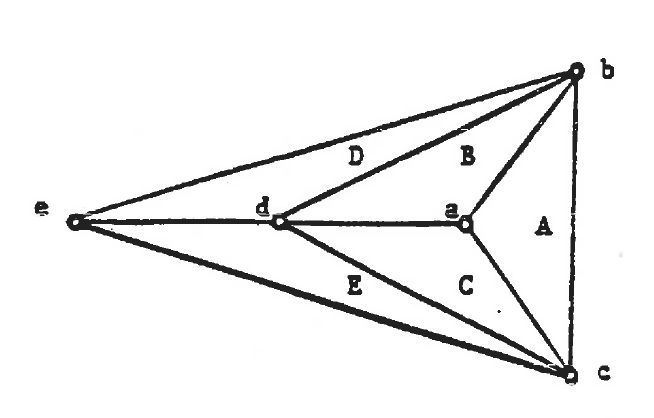
\includegraphics[width=.62\textwidth]{images/fig1.png}\par 图1\end{center}
\src{3}
设 $\Delta$ 为纯单纯复形。它的一个\textbf{壳序}是刻面的线性次序，使每个刻面与此前刻面生成的复形的交，是其若干极大真面的非空并。\redinsert{也就是说，新刻面沿若干完整的余维一面贴入，而不是只沿孤立的低维面贴入。}换言之，刻面的线性次序 $F_1,\ldots,F_t$ 是壳序，当且仅当
\[\begin{gathered}
\text{对每对 }F_i,F_j\ (1\le i<j\le t),\text{存在 }F_k\ (1\le k<j)\text{ 及 }x\in F_j,\\
F_i\cap F_j\subseteq F_k\cap F_j=F_j-x.
\end{gathered}\tag{7.3}\]
纯复形若有壳序，称为\textbf{可壳}的。每个零维复形都可壳；一维复形（简单图）可壳当且仅当连通。壳序的直观含义是：逐次加入刻面来构造纯 $d$ 维复形，每次把新刻面很好地贴到已构造部分上，使交在拓扑上是 $(d-1)$ 维球或 $(d-1)$ 维球面。
图1中，先将 $A,B,C$ 任意排列，再将 $D,E,F$ 任意排列，便得到壳序；但以 $A,B,E,\ldots$ 或 $D,E,C,A,\ldots$ 开始的次序不是壳序。
本节余下部分固定以下记号：$\Delta$ 是 $(r-1)$ 维可壳复形，$F_1,\ldots,F_t$ 按壳序排列。令 $\Delta_i=\{G\in\Delta:G\subseteq F_k\text{ 对某个 }k\le i\}$，即前 $i$ 个刻面生成的子复形。对 $i=1,\ldots,t$，令 $\RR(F_i)=\{x\in F_i:F_i-x\in\Delta_{i-1}\}$，称为壳序诱导的 $F_i$ 的\textbf{限制面}。\redinsert{（删去其中任一顶点后，剩下的面都已在先前出现。）}于是 $\RR(F_i)=\varnothing$ 当且仅当 $i=1$；$\RR(F_i)=F_i$ 当且仅当其所有真子集都属于 $\Delta_{i-1}$。把 $\Delta$ 按面的包含关系排序，可在其中考虑布尔区间 $[G_1,G_2]=\{G:G_1\subseteq G\subseteq G_2\}$。
\st{命题7.2.2}区间 $[\RR(F_i),F_i]$（$i=1,\ldots,t$）划分可壳复形 $\Delta$。
\pr $F_1,\ldots,F_i$ 是 $\Delta_i$ 的壳序，故归纳地只需证明：(i) $\Delta_{t-1}\cup[\RR(F_t),F_t]=\Delta$；(ii) $\Delta_{t-1}\cap[\RR(F_t),F_t]=\varnothing$。若 $G\in\Delta-\Delta_{t-1}$，则 $G\subseteq F_t$。若某个 $x\in\RR(F_t)$ 不属于 $G$，则 $G\subseteq F_t-x\in\Delta_{t-1}$，矛盾。因此 $\RR(F_t)\subseteq G$，得到(i)。(ii)等价于 $\RR(F_t)\notin\Delta_{t-1}$。若不然，则对某个 $i<t$，$\RR(F_t)\subseteq F_i\cap F_t$。由(7.3)，存在 $k<t$ 及 $x\in F_t$，使 $\RR(F_t)\subseteq F_i\cap F_t\subseteq F_k\cap F_t=F_t-x$。
\src{4}
然而 $F_t-x\subseteq F_k\in\Delta_{t-1}$ 蕴含 $x\in\RR(F_t)$，与 $\RR(F_t)\subseteq F_t-x$ 矛盾。\qed
这表明：在壳化过程中把刻面 $F_i$ 及其子面加入 $\Delta_{i-1}$ 时，$\RR(F_i)$ 是 $F_i$ 中唯一极小的“新”面，即属于 $\Delta_i-\Delta_{i-1}$ 的极小面。\redinsert{换言之，本步新增的恰是 $F_i$ 中包含整个 $\RR(F_i)$ 的那些子面。}定义可壳复形的\textbf{壳多项式}
\[h_\Delta(x)=\sum_{i=1}^t x^{|F_i-\RR(F_i)|}.\tag{7.4}\]
\st{命题7.2.3}若 $\Delta$ 可壳，则 $h_\Delta(1+\lambda)=f_\Delta(\lambda)$。因此壳多项式与壳序选择无关。
\pr 由二项式展开，
\[\begin{aligned}
h_\Delta(1+\lambda)&=\sum_i(1+\lambda)^{|F_i-\RR(F_i)|}\\
&=\sum_i\sum_{k=0}^r\binom{|F_i-\RR(F_i)|}{k}\lambda^k
=\sum_{k=0}^r\left(\sum_i\binom{|F_i-\RR(F_i)|}{k}\right)\lambda^k.
\end{aligned}\]
由命题7.2.2，$f_{r-k}=\sum_i\binom{|F_i-\RR(F_i)|}{k}$。\redinsert{这是因为每块中的面必须保留限制面；要得到大小为 $r-k$ 的面，只需从其余顶点中删去 $k$ 个。}\qed
所以 $h_\Delta(1)$ 等于刻面数，$h_\Delta(2)$ 等于总面数。更重要的是 $h_\Delta(0)=f_\Delta(-1)=(-1)^{r-1}\chi(\Delta)$。另一方面，由定义它等于满足 $\RR(F)=F$ 的刻面数。因此：
\st{推论7.2.4}$(-1)^{r-1}\chi(\Delta)$ 等于满足 $\RR(F)=F$ 的刻面 $F$ 的个数。\qed
取例7.2.1中的壳序 $A,B,C,D,E,F$，有 $\RR(A)=\varnothing$、$\RR(B)=\{d\}$、$\RR(C)=\{c,d\}$、$\RR(D)=\{e\}$、$\RR(E)=\{c,e\}$、$\RR(F)=F$。故
\[h_\Delta(x)=x^3+x^2+x+x^2+x+1=x^3+2x^2+2x+1.\]
可检验 $h_\Delta(2)=21$ 是总面数，$h_\Delta(1)=6$ 是刻面数，$h_\Delta(0)=1$ 等于欧拉示性数；而 $h_\Delta(1+\lambda)=\lambda^3+5\lambda^2+9\lambda+6=f_\Delta(\lambda)$。
写 $f_\Delta(\lambda)=\sum_{i=0}^rf_i\lambda^{r-i}$，$h_\Delta(x)=\sum_{i=0}^rh_ix^{r-i}$。称 $(f_0,\ldots,f_r)$ 和 $(h_0,\ldots,h_r)$ 分别为 $f$ 向量和 $h$ 向量。它们密切相关。比较 $f_\Delta(\lambda)=h_\Delta(1+\lambda)$ 的系数，得到
\[f_k=\sum_{i=0}^rh_i\binom{r-i}{k-i},\qquad k=0,\ldots,r.\tag{7.5}\]
\src{5}
类似地，由 $h_\Delta(x)=f_\Delta(x-1)$ 得逆公式
\[h_k=\sum_{i=0}^r(-1)^{i+k}f_i\binom{r-i}{k-i},\qquad k=0,\ldots,r.\tag{7.6}\]
因此 $h_0=f_0=1$，$h_1=f_1-r$。这也可直接由(7.4)得到，其等价表述为
\[h_k=\#\{\text{刻面 }F:|\RR(F)|=k\},\qquad0\le k\le r.\tag{7.7}\]
故所有 $h_k\ge0$。\redinsert{（$h_k$ 按限制面的大小计数，$f_k$ 则按面的大小计数。）}下面用 $f$ 向量与 $h$ 向量的关系研究可壳复形的若干计数事实，它们仅用于第7.5节。
\st{命题7.2.5}设 $\Delta$ 是顶点集 $V$ 上的 $(r-1)$ 维可壳复形，$|V|=v>r$。则：
\begin{enumerate}[label=(\roman*)]
\item 对所有 $0\le k<j\le r-k$，有 $f_k<f_j$。
\item 若 $1\le k<(r+1)/2$ 且 $h_{r-k+1}\ge1$，则 $f_k\le f_{r-k+1}$；等号成立当且仅当还满足 $h_2=1$。
\item 若 $V$ 的所有 $e$ 元子集均属于 $\Delta$，其中 $e<r$，则
\[f_k\ge\sum_{i=0}^e\binom{v-r+i-1}{i}\binom{r-i}{k-i},\qquad k=0,\ldots,r.\]
而且下列条件等价：$(\alpha)$ 对某个 $k>e$ 等号成立；$(\beta)$ 对所有 $k$ 等号成立；$(\gamma)$ $f_r=\binom{v-r+e}{e}$。
\end{enumerate}
\pr (i)直接由(7.5)、(7.7)中的非负性和二项式系数的初等性质得到。(ii)需要进一步使用 $h$ 向量的结构，见习题7.2.2。
对(iii)，假设所有 $e$ 元子集都是面，即 $f_k=\binom vk$（$k=0,\ldots,e$）。用恒等式 $(-1)^y\binom{-x}{y}=\binom{x+y-1}{y}$ 和 Vandermonde 卷积 $\binom{x+y}k=\sum_i\binom xi\binom y{k-i}$，由(7.6)，对 $k\le e$ 得
\[\begin{aligned}
h_k&=\sum_{i=0}^k(-1)^{i+k}\binom{r-i}{k-i}\binom vi\\
&=\sum_{i=0}^k\binom{k-r-1}{k-i}\binom vi=\binom{v-r+k-1}k.
\end{aligned}\tag{7.8}\]
代入(7.5)，并用 $k>e$ 时的 $h_k\ge0$，保留前 $e+1$ 项即得不等式。同一论证说明，若 $(\delta)$ $h_{e+1}=\cdots=h_r=0$，则所有 $k$ 都取等。因此 $(\delta)\Rightarrow(\beta)\Rightarrow(\gamma)\Rightarrow(\alpha)$，其中$(\gamma)$就是 $k=r$ 时取等。若某个 $k>e$ 取等，(7.5)给出 $h_{e+1}=\cdots=h_k=0$。
\src{6}
由下述引理结合(7.7)，其后的 $h_{k+1},\ldots,h_r$ 也均为零，故 $(\alpha)\Rightarrow(\delta)$。\redinsert{若存在更大的限制面，反复使用引理删去元素就会得到大小为 $k$ 的限制面，与 $h_k=0$ 矛盾。}\qed
\st{引理7.2.6}设 $\mathcal F=\{\RR(F_i):1\le i\le t\}$，其中 $F_1,\ldots,F_t$ 是 $\Delta$ 的壳序。则对任意 $A\in\mathcal F-\{\varnothing\}$，存在 $x\in A$ 使 $A-x\in\mathcal F$。
\pr 设 $1<g\le t$，令 $X_1,\ldots,X_s$ 是 $\RR(F_g)$ 的极大真子集。由于 $\RR(F_g)$ 是 $\Delta_g-\Delta_{g-1}$ 中唯一极小面，它们都属于 $\Delta_{g-1}$。由命题7.2.2，存在唯一的刻面 $F_{i_j}$，使 $\RR(F_{i_j})\subseteq X_j\subseteq F_{i_j}$ 且 $i_j<g$。不同 $j,k$ 对应不同刻面；否则 $\RR(F_g)=X_j\cup X_k\subseteq F_{i_j}$，与命题7.2.2矛盾。不妨 $i_1<\cdots<i_s$。$X_s$ 的每个真子集都属于 $\Delta_{i_s-1}$，故 $\RR(F_{i_s})$ 不可能真包含于 $X_s$。因此 $\RR(F_{i_s})=X_s\subset\RR(F_g)$，且 $|\RR(F_g)|=|\RR(F_{i_s})|+1$。\qed

\sect{7.3\quad 拟阵复形}
若 $M=M(S)$ 是有限集 $S$ 上秩为 $r$ 的拟阵，其全部独立集构成 $(r-1)$ 维单纯复形，记为 $\IN(M)$，称为\textbf{拟阵复形}。\redinsert{（刻面恰是拟阵的基，所以所有刻面的大小都等于秩 $r$。）}拟阵复形是纯的是拟阵理论的基本事实；我们很快将看到它也可壳。事实上，拟阵复形既可用纯性刻画，也可用可壳性刻画（习题7.3.1和定理7.3.4）。
给底层点集一个线性次序，会揭示拟阵的一些重要性质，而这些性质本身不依赖次序。\textbf{有序拟阵} $M(S,\omega)$ 指拟阵 $M(S)$ 连同 $S$ 上的线性次序 $\omega$。约定将 $k$ 元子集按 $x_1<\cdots<x_k$ 写为 $[x_1,\ldots,x_k]$。其\textbf{字典序}定义为：若某个位置 $e$ 满足 $x_i=y_i$（$i<e$）且 $x_e<y_e$，则 $[x_1,\ldots,x_k]$ 排在 $[y_1,\ldots,y_k]$ 之前。下文比较基时均使用此诱导次序。
回忆：若 $B$ 是基且 $p\in S-B$，则 $B\cup p$ 含唯一回路 $\ci(B,p)$；\redinsert{（$B\cup p$ 表示 $B\cup\{p\}$，下文 $B-b$ 类似表示删去单个元素。）}对偶地，若 $b\in B$，则 $(S-B)\cup b$ 含唯一余回路（bond）$\bo(B,b)$。\redinsert{（余回路就是对偶拟阵的回路。）}基本回路和基本余回路满足：
\st{引理7.3.1}$b\in\ci(B,p)\Longleftrightarrow(B-b)\cup p\text{ 是基}\Longleftrightarrow p\in\bo(B,b)$。
设 $C$ 是有序拟阵的回路，$c$ 是其中最小元素，则 $C-c$ 称为\textbf{断路}。不含任何断路的基称为\textbf{nbc基}。这个概念在后续各节十分重要；这里先在下面的技术引理中使用，它是本节和下一节的关键。
\st{引理7.3.2}设 $M(S,\omega)$ 是有序拟阵，基 $B$ 在字典序中先于基 $C$。则存在也先于 $C$ 的基 $A$，使 $B\cap C\subseteq A\cap C$ 且 $|A\cap C|=|C|-1$。此外，若 $C$ 是nbc基，可选择 $A$ 也是nbc基。
\pr 设 $B=[b_1,\ldots,b_r]$、$C=[c_1,\ldots,c_r]$，且 $b_i=c_i$（$i<e$）、$b_e\ne c_e$。则 $b_e<c_i$（$i=e,\ldots,r$）。由基交换性质，存在 $y\in C-B$，使 $A_1=(C-y)\cup b_e$ 为基。第一条结论可取 $A=A_1$。
\src{7}
对第二条，设 $C$ 是nbc基。若 $A_1$ 不是nbc基，则存在 $a_1\in S-A_1$，它是基本回路 $\ci(A_1,a_1)$ 的最小元素。$b_e$ 必属于此回路，否则 $C$ 将包含断路 $\ci(A_1,a_1)-a_1$。因此 $A_2=(A_1-b_e)\cup a_1$ 是基，且先于 $A_1$，满足 $B\cap C\subseteq A_2\cap C$、$|A_2\cap C|=r-1$。若 $A_2$ 仍不是nbc基，就重复此过程，有限步后得到所需的 $A=A_k$。\redinsert{每次基的字典序都严格下降，而基的个数有限，因此过程必定终止。}\qed
去掉关于nbc基的最后一句，引理7.3.2等价于以下结果（比较(7.3)）：
\st{定理7.3.3}有序拟阵 $M(S,\omega)$ 的基的 $\omega$ 字典序是 $\IN(M)$ 的壳序。特别地，所有拟阵复形都可壳。
因此底集的每个线性次序都诱导壳序，这种丰富性实际上刻画了拟阵。
\st{定理7.3.4}单纯复形 $\Delta$ 是拟阵复形，当且仅当它纯，且顶点的每个排序都诱导壳序。\redinsert{这里要求每个排序都成立；仅有一个排序给出壳序，并不足以刻画拟阵。}
\pr 必要性即定理7.3.3。反之，设纯复形 $\Delta$ 不是拟阵复形。存在 $U\subseteq V$，使诱导子复形 $\Delta_U=\{F\in\Delta:F\subseteq U\}$ 不纯（习题7.3.1）。取其最小维刻面 $F$；在维数大于 $\dim F$ 的刻面中，取使 $|F\cap G|$ 尽可能大的 $G$。将顶点排为：$F-G$ 在前，$G$ 次之，其余在后。令 $\widetilde G$ 为首个包含 $G$ 的刻面，$\widetilde F$ 为任意包含 $F$ 的刻面。由极大性，$\widetilde F\cap U=F$，$\widetilde G\cap U=G$。所选次序保证：刻面 $H$ 先于 $\widetilde G$ 当且仅当 $H\cap(F-G)\ne\varnothing$。特别地，$\widetilde F$ 先于 $\widetilde G$。由于 $F,G$ 是 $\Delta_U$ 的刻面且 $|F|<|G|$，有 $|F\cap G|\le|G|-2$，故 $|\widetilde F\cap\widetilde G|\le|\widetilde G|-2$。
若有先于 $\widetilde G$ 的刻面 $H$ 和 $g\in\widetilde G$ 满足 $\widetilde F\cap\widetilde G\subseteq H\cap\widetilde G=\widetilde G-g$，则 $g\in\widetilde G-\widetilde F$，且 $H-\widetilde G=\{h\}$，$h\in F-G$。若 $g\in\widetilde G-G$，则 $G\cup h\subseteq H\cap U$，与 $G$ 极大矛盾。若 $g\in G-F$，则 $G'=(G-g)\cup h$ 是 $\Delta_U$ 中维数等于 $\dim G>\dim F$ 的面，且 $|F\cap G'|>|F\cap G|$，与 $G$ 的选择矛盾。因此无此 $H$，所诱导次序不是壳序。\qed
现在求壳多项式。若 $p\in S-B$ 是 $\ci(B,p)$ 的最小元素，称其在 $B$ 中\textbf{外活跃}，否则称外被动。对偶地，若 $p\in B$ 是 $\bo(B,p)$ 的最小元素，称其\textbf{内活跃}，否则称内被动。\redinsert{（由引理7.3.1，内被动意味着该元素可被某个更小的基外元素替换。）}分别用 $\EA(B),\EP(B),\IA(B),\IP(B)$ 记这四类元素集。称 $i(B)=|\IA(B)|$ 为内活性，$e(B)=|\EA(B)|$ 为外活性。显然 $p$ 在 $B$ 中内活跃，当且仅当它在对偶有序拟阵 $M^*(S,\omega)$ 的基 $S-B$ 中外活跃。
\st{例7.3.5}设 $M$ 是图2(a)仿射空间中点线关系所定义的拟阵，也等价于图2(b)的图拟阵。
\src{8}
\begin{center}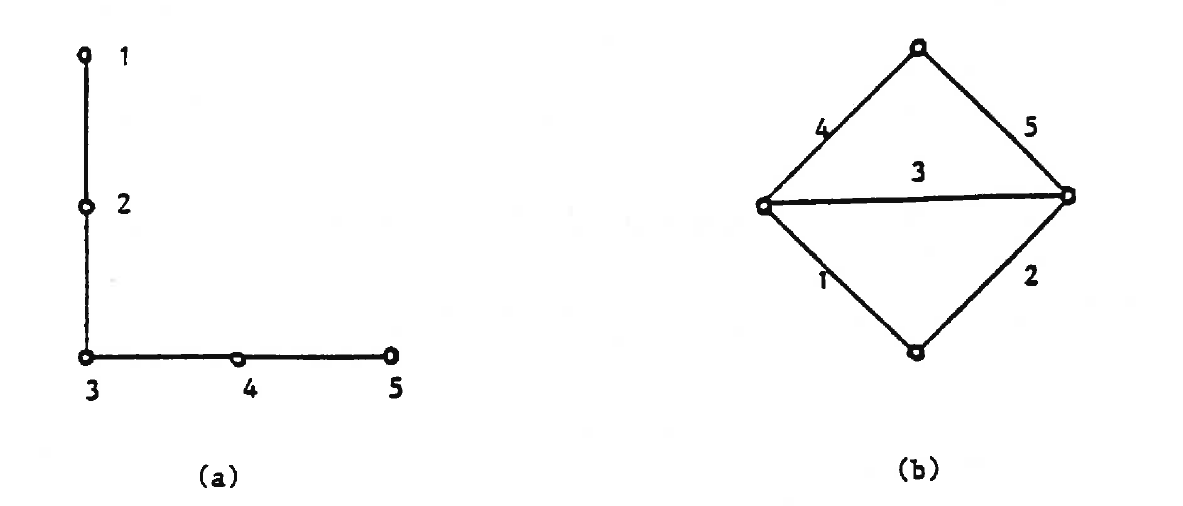
\includegraphics[width=.8\textwidth]{images/fig2.png}\par 图2\end{center}
将8个基按字典序列出，并标明各基的活跃元素：
\begin{center}\begin{tabular}{ccc}\toprule 基&内活跃元素&外活跃元素\\\midrule
$B_1=[1,2,4]$&$1,2,4$&无\\
$B_2=[1,2,5]$&$1,2$&无\\
$B_3=[1,3,4]$&$1,4$&无\\
$B_4=[1,3,5]$&$1$&无\\
$B_5=[1,4,5]$&$1$&$3$\\
$B_6=[2,3,4]$&$4$&$1$\\
$B_7=[2,3,5]$&无&$1$\\
$B_8=[2,4,5]$&无&$1,3$\\\bottomrule\end{tabular}\end{center}
$\IN(M)$ 的图像见图3：它是三角双锥的表面，加上内部两个三角形145和245。观察基序列 $B_1,\ldots,B_8$ 怎样给出壳序，颇有启发。
\begin{center}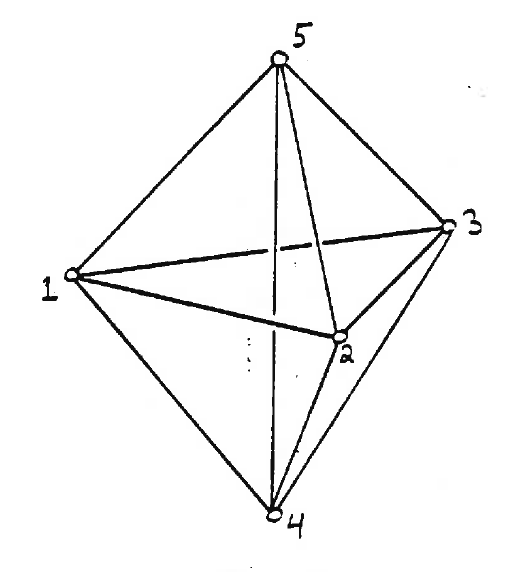
\includegraphics[width=.46\textwidth]{images/fig3.png}\par 图3\end{center}
\src{9}
再考虑有序拟阵基的字典序。由引理7.3.1，$B-b$ 包含于一个先于 $B$ 的基，当且仅当 $b$ 在 $B$ 中内被动。\redinsert{确实，替换成更小元素便得到字典序更早的基；反过来，更早的基也提供这样的替换。}因此
\[\RR(B)=\IP(B).\tag{7.9}\]
所以拟阵复形 $\Delta=\IN(M)$ 的壳多项式为
\[h_\Delta(x)=\sum_Bx^{|B-\RR(B)|}=\sum_Bx^{|\IA(B)|}=\sum_Bx^{i(B)}.\tag{7.10}\]
对偶地，$\Delta^*=\IN(M^*)$ 的壳多项式为 $h_{\Delta^*}(y)=\sum_By^{e(B)}$。两处都对 $M$ 的全部基求和。因此很自然将二者合成二元多项式
\[T_M(x,y)=\sum_Bx^{i(B)}y^{e(B)}.\tag{7.11}\]
但有一个困难：我们由命题7.2.3知道
\[T_M(x,1)=h_{\IN(M)}(x),\qquad T_M(1,y)=h_{\IN(M^*)}(y)\tag{7.12}\]
与次序无关，却不能立即知道 $T_M(x,y)$ 本身与次序无关。下面将证明这一点，故称为 $M$ 的\textbf{Tutte多项式}的 $T_M$ 只依赖拟阵结构。
先回到例7.3.5。由活跃元素表得
\[\begin{aligned}
T_M(x,y)&=x^3+x^2+x^2+x+xy+xy+y+y^2\\
&=x^3+2x^2+y^2+2xy+x+y.
\end{aligned}\]
因此 $h_{\IN(M)}(x)=x^3+2x^2+3x+2$，而 $h_{\IN(M^*)}(y)=y^2+3y+4$。
\st{命题7.3.6}对有序拟阵 $M(S,\omega)$，每个基 $B$ 对应的区间 $[\IP(B),S-\EP(B)]$ 划分布尔代数 $2^S$。\redinsert{在这个区间中，内被动元素必须保留，外被动元素必须排除，其余元素可自由选取；这里也包括相关集。}
\pr 需证明每个 $A\subseteq S$ 存在唯一基 $B_A$，使 $\IP(B_A)\subseteq A\subseteq S-\EP(B_A)$。
\src{10}
令 $X_A$ 是限制拟阵 $M_A$ 的字典序最大基。由命题7.2.2及(7.9)，存在唯一的 $M$ 的基 $B_A$，使 $\IP(B_A)\subseteq X_A\subseteq B_A$。取 $a\in A-B_A=A-X_A$，反设它在 $B_A$ 中外被动，则有 $b\in B_A$，使 $b<a$ 且 $(B_A-b)\cup a$ 是基。若 $b\notin A$，则 $X_A\cup a$ 独立，与 $X_A$ 是 $M_A$ 的基矛盾。若 $b\in A$，则 $b\in B_A\cap A=X_A$，且 $(X_A-b)\cup a$ 是字典序更大的基，仍矛盾。因此 $A-B_A$ 中所有元素都外活跃，从而 $\IP(B_A)\subseteq X_A\subseteq A\subseteq S-\EP(B_A)$。
再设某基 $B$ 满足 $\IP(B)\subseteq A\subseteq S-\EP(B)$。注意
\[\EA(B)\subseteq\operatorname{cl}(\IP(B)).\tag{7.13}\]
事实上，若 $p\in S-B$ 外活跃，令 $C=\ci(B,p)$，$C'=C-p$。对每个 $q\in C'$，$p<q$ 且 $(B-q)\cup p$ 为基，所以 $q$ 内被动。又 $p\in\operatorname{cl}(C')$，$C'\subseteq\IP(B)$，故(7.13)成立。这说明 $X=B\cap A$ 是 $M_A$ 的基。
若 $X\ne X_A$，写 $X=\{x_1<\cdots<x_a\}$、$X_A=\{y_1<\cdots<y_a\}$。由 $X_A$ 最大，存在 $e$ 使 $x_i=y_i$（$i<e$），且 $x_e<y_i$（$i\ge e$）。由基交换公理，某个 $j\ge e$ 使 $(X-x_e)\cup y_j$ 为基。于是 $y_j$ 在 $X$ 中外被动，因而在 $B$ 中也外被动，与 $A\subseteq S-\EP(B)$ 矛盾。因此 $X=X_A$，再由 $\IP(B)\subseteq X\subseteq B$ 得 $B=B_A$。\qed
\st{定理7.3.7}对有序拟阵 $M$，有
\[T_M(1+\xi,1+\eta)=\sum_{A\subseteq S}\xi^{r(S)-r(A)}\eta^{r^*(S)-r^*(S-A)},\]
其中 $r,r^*$ 分别为 $M,M^*$ 的秩函数。特别地，Tutte多项式与 $S$ 的次序无关。\redinsert{因为右侧只使用秩函数，并未使用次序；由对偶秩公式，第二个指数还可写成 $|A|-r(A)$。}
\pr 若 $\IP(B)\subseteq A\subseteq S-\EP(B)$，(7.13)给出 $r(A)=|A\cap B|$，故 $r(S)-r(A)=|B-A|$；对偶地，$r^*(S)-r^*(S-A)=|(S-B)-(S-A)|=|A-B|$。由命题7.3.6，
\[\begin{aligned}
\sum_{A\subseteq S}\xi^{r(S)-r(A)}\eta^{r^*(S)-r^*(S-A)}
&=\sum_{B\text{ 为基}}\sum_{\IP(B)\subseteq A\subseteq S-\EP(B)}\xi^{|B-A|}\eta^{|A-B|}\\
&=\sum_B\sum_{j,k\ge0}\binom{i(B)}j\binom{e(B)}k\xi^j\eta^k\\
&=\sum_B(1+\xi)^{i(B)}(1+\eta)^{e(B)}=T_M(1+\xi,1+\eta).
\end{aligned}\]\qed
\src{11}
本卷第6章详细讨论Tutte多项式，更多内容可参阅那里。本节结束前指出，由(7.12)和推论7.2.4，$\chi(\IN(M))=(-1)^{r-1}T_M(0,1)$。命题7.4.7将给出另一表达式。

\sect{7.4\quad 断路复形}
设 $M=M(S,\omega)$ 是有序拟阵。回忆：从回路中删去最小元素，所得集合称为断路。\redinsert{例如回路 $\{1,2,3\}$ 在 $1<2<3$ 下给出断路 $\{2,3\}$；它本身独立，却被断路复形额外排除。}$S$ 中所有不含断路的子集组成的单纯复形记为 $\BC_\omega(M)$，称为 $M$ 的\textbf{断路复形}。注意它有定义当且仅当 $M$ 无环；若有环，则每个子集都含断路 $\varnothing$。
讨论断路复形时，除环外，方便时也可排除平行元素。无环拟阵中若 $r_M(\{x,y\})=1$，称 $x,y$ 平行。平行是等价关系。在等价类集 $\bar S$ 上定义秩函数 $r_{\bar M}(\{X_1,\ldots,X_n\})=r_M(X_1\cup\cdots\cup X_n)$，得到无环且无平行元素的拟阵 $\bar M(\bar S)$，称为 $M$ 的\textbf{简化}。若 $M(S,\omega)$ 有序，按各平行类的最小元素给 $\bar S$ 排序，记为 $\bar\omega$。有如下直接观察：
\st{命题7.4.1}断路复形 $\BC_\omega(M)$ 与 $\BC_{\bar\omega}(\bar M)$ 同构。\redinsert{若 $x<y$ 平行，则 $\{x,y\}$ 是回路，$\{y\}$ 是断路，故每个平行类只留下最小代表。}\qed
需要解释次序在构造中的作用：同一拟阵的不同点序，可能给出不同构的断路复形，例7.4.4将予以展示；但其重要不变量与次序无关。
设无环有序拟阵 $M(S,\omega)$ 的最小元素为 $e$。$S-e$ 中所有不含断路的子集组成\textbf{约化断路复形}，记为 $\overline{\BC}_\omega(M)$。先列出基本观察。
\st{命题7.4.2}设 $M(S,\omega)$ 无环且秩为 $r$。则：
\begin{enumerate}[label=(\roman*)]
\item $\overline{\BC}_\omega(M)\subseteq\BC_\omega(M)\subseteq\IN(M)$；
\item $\BC_\omega(M)$ 是纯 $(r-1)$ 维复形，其刻面为 $M$ 的nbc基；
\item $\BC_\omega(M)$ 是以 $e$ 为锥顶、以 $\overline{\BC}_\omega(M)$ 为底的锥；
\item $\overline{\BC}_\omega(M)$ 是纯 $(r-2)$ 维复形。
\end{enumerate}
\pr 若 $X\subseteq S$ 不含断路，则更不含回路，因此独立。\redinsert{因为任一回路都包含删去其最小元素所得到的断路。}令 $B$ 为包含 $X$ 的字典序最小基。若 $B$ 含断路 $C$，则可找到 $y,z\in S$，使 $y\notin B$、$C\cup y=\ci(B,y)$、$z\in C-X$ 且 $y<z$。于是 $(B-z)\cup y$ 是包含 $X$ 而先于 $B$ 的基，矛盾。所以 $B$ 是nbc基，得到(i)、(ii)。若基 $B$ 不含最小元素 $e$，则它含断路 $\ci(B,e)-e$。因此所有nbc基都含 $e$，得到(iii)、(iv)。\redinsert{任一面都包含于某个nbc基，因而也能加入 $e$ 而仍是面，这正是锥的性质。}\qed
若 $B$ 是nbc基，称 $B-e$ 为\textbf{约化nbc基}。下面是本节的基本结果。
\src{12}
\st{定理7.4.3}若 $M(S,\omega)$ 无环，则 $\BC_\omega(M)$ 和 $\overline{\BC}_\omega(M)$ 都可壳。两者的刻面（分别为nbc基、约化nbc基）的 $\omega$ 字典序都是壳序。
\pr 对 $\BC_\omega(M)$，引理7.3.2已证明。由命题7.4.2(iii)和习题7.2.1，约化复形的结论随之成立。\qed
\st{例7.4.4}考虑例7.3.5中 $S=\{1,2,3,4,5\}$ 上的拟阵。自然次序 $\omega$ 下，断路为 $\{2,3\}$、$\{4,5\}$、$\{2,4,5\}$；nbc基为 $\{1,2,4\}$、$\{1,2,5\}$、$\{1,3,4\}$、$\{1,3,5\}$。在次序 $\omega':1<2<4<3<5$ 下，断路为 $\{2,3\}$、$\{3,5\}$、$\{2,4,5\}$；nbc基为 $\{1,2,4\}$、$\{1,2,5\}$、$\{1,3,4\}$、$\{1,4,5\}$。所以两个断路复形不同构，其约化复形见图4。也可观察两种情况下边的相应字典序如何给出壳序。
\begin{center}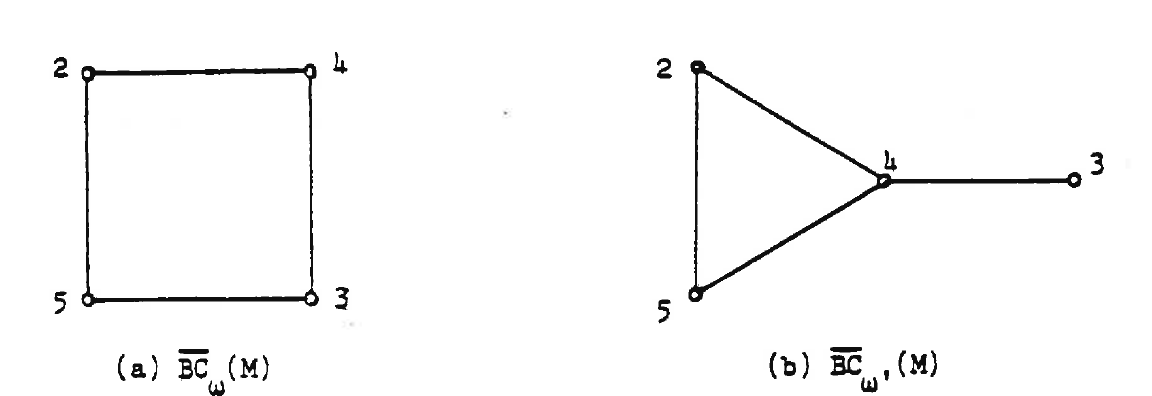
\includegraphics[width=.85\textwidth]{images/fig4.png}\par 图4\end{center}
现在转向壳多项式及计数性质。设 $B$ 是nbc基且 $b\in B$。若 $B-b$ 包含于字典序更小的nbc基，则如(7.9)，$b\in\IP(B)$。反之若 $b$ 内被动，则 $B-b$ 包含于某个先于 $B$ 的基；命题7.4.2的证明说明，包含 $B-b$ 的最早基是nbc基。因此在断路复形的字典壳序中，
\[\RR(B)=\IP(B).\tag{7.14}\]
故壳多项式等于对nbc基求和的 $\sum_Bx^{i(B)}$。而 $B$ 不含断路当且仅当 $e(B)=0$，所以\redinsert{（在 $T_M(x,y)$ 中令 $y=0$，恰好只保留外活性为零的基。）}
\[h_{\BC_\omega(M)}(x)=T_M(x,0).\tag{7.15}\]
类似推理可直接得到，或由命题7.4.2(iii)、习题7.2.1及(7.15)得到，约化断路复形的壳多项式为\redinsert{（删去的最小元素 $e$ 在每个nbc基中都是内活跃的，故壳多项式少一个因子 $x$）}
\[h_{\overline{\BC}_\omega(M)}(x)=\frac1xT_M(x,0).\tag{7.16}\]
\src{13}
由(7.15)，断路复形的面数与次序无关。例7.4.4中两个不同构复形的 $f$ 向量都是 $(1,5,8,4)$。
断路复形的面数及面枚举多项式 $T_M(1+\lambda,0)$ 是拟阵理论中十分有趣的数值不变量。以下假定读者熟悉秩 $r$ 几何格的Möbius函数 $\mu(x,y)$ 和特征多项式
\[p(L;\lambda)=\sum_{x\in L}\mu(\hat0,x)\lambda^{r-r(x)}=\sum_{k=0}^rw_k\lambda^{r-k}.\]
参见 White (1987) 第7、8章或 Stanley (1986)。非负整数 $\widetilde w_k=(-1)^kw_k$ 称为（无符号的）\textbf{第一类Whitney数}。
\st{命题7.4.5}设 $M(S,\omega)$ 是无环有序拟阵，$L$ 是相应几何格。对 $x\in L$，令 $\nbc(x)=\{A\in\BC_\omega(M):\bar A=x\}$，则\redinsert{（$\bar A$ 是 $A$ 的闭包，即它张成的平坦集；这里把面按闭包分类）}
\[|\nbc(x)|=(-1)^{r(x)}\mu(\hat0,x).\]
\pr 证明 $(-1)^{r(y)}|\nbc(y)|$ 与 $\mu(\hat0,y)$ 满足同一递推。仅空集张成空平坦集，故 $|\nbc(\hat0)|=1$。设 $x\ne\hat0$，令 $S'$ 为平坦集 $x$ 上的点集，$M'(S',\omega')$ 为相应限制。$S'$ 的子集在 $M'$ 中为断路当且仅当在 $M$ 中为断路。因此 $\BC_{\omega'}(M')=\bigcup_{y\le x}\nbc(y)$，且为无交并。$\nbc(y)$ 的每个元素既独立又张成 $y$，故基数为 $r(y)$。又因 $\BC_{\omega'}(M')$ 是锥，由(7.2)，
\[\sum_{\hat0\le y\le x}(-1)^{r(y)}|\nbc(y)|=-\chi(\BC_{\omega'}(M'))=0.\]
证明完成。\qed
把命题两侧对秩为 $k$ 的平坦集求和，左边得到无断路 $k$ 元子集总数，右边得到 $\widetilde w_k$。于是：
\st{定理7.4.6}无环拟阵的第一类Whitney数，等于任意次序诱导的断路复形的面数。
结合(7.15)和命题7.2.3，可写为
\[p(M;\lambda)=(-1)^rh_{\BC_\omega(M)}(1-\lambda)=(-1)^rT_M(1-\lambda,0).\tag{7.17}\]
例7.3.5中，已算得 $T_M(x,y)=x^3+2x^2+y^2+2xy+x+y$，所以 $T_M(1-\lambda,0)=4-8\lambda+5\lambda^2-\lambda^3=-p(M;\lambda)$。这与其断路复形的 $f$ 向量 $(1,5,8,4)$ 相符。
本节最后确定拟阵复形及（约化）断路复形的欧拉示性数。需要拟阵 $M(S)$ 的\textbf{beta不变量}\redinsert{（这是拟阵的不变量，勿与一般的 Betti 数混淆）}
\[\beta(M)=(-1)^{r(S)}\sum_{A\subseteq S}(-1)^{|A|}r(A),\tag{7.18}\]
其讨论见 White (1987) 第7章。再定义\textbf{Möbius不变量}
\[\widetilde\mu(M)=\begin{cases}|\mu_L(\hat0,\hat1)|,&M\text{ 无环},\\0,&M\text{ 有环},\end{cases}\tag{7.19}\]
其中第一种情形的 $L$ 是 $M$ 的平坦集格。显然 $\widetilde\mu(M)=\widetilde w_r(L)$。
\src{14}
\st{命题7.4.7}设 $M$ 秩为 $r$，在(ii)、(iii)中还假定无环且按 $\omega$ 排序。则
\begin{enumerate}[label=(\roman*)]
\item $\chi(\IN(M))=(-1)^{r-1}\widetilde\mu(M^*)$；
\item $\chi(\BC_\omega(M))=0$；
\item $\chi(\overline{\BC}_\omega(M))=(-1)^r\beta(M)$。
\end{enumerate}
\pr (ii)由锥性质立即得到。\redinsert{这里 $\chi$ 始终表示约化欧拉示性数，所以锥的值为零。}其余用推论7.2.4的 $\chi(\Delta)=(-1)^{r-1}h_\Delta(0)$。对(i)，当 $M^*$ 无环时，(7.12)、(7.17)给出
\[h_{\IN(M)}(0)=T_M(0,1)=T_{M^*}(1,0)=(-1)^{n-r}p(M^*;0)=\widetilde\mu(M^*).\]
若 $M^*$ 有环，则 $\IN(M)$ 是锥，两边都是零。对(iii)，由(7.16)和定理7.3.7，
\[\begin{aligned}
h_{\overline{\BC}_\omega(M)}(0)&=\frac{\partial T_M}{\partial x}(0,0)\\
&=\sum_{A\subseteq S}(r(S)-r(A))(-1)^{r(S)-r(A)-1+r^*(S)-r^*(S-A)}\\
&=(-1)^{r(S)}\sum_{A\subseteq S}(r(A)-r(S))(-1)^{|A|}=\beta(M).
\end{aligned}\]\qed
由此对所有拟阵有 $\beta(M)\ge0$。为后续使用，列出下述性质；证明见 White (1987) 第7章。
\st{命题7.4.8}对任意 $|S|\ge2$ 的拟阵 $M(S)$：(i) $\beta(M)=\beta(M^*)$；(ii) $\beta(M)>0$ 当且仅当 $M$ 连通。

\sect{7.5\quad 拟阵不等式的应用}
前面建立的材料为处理独立数及第一类Whitney数的某些不等式提供了良好框架。本节专论此应用；跳过本节也不影响后续连贯性。在这些不等式背后，是理解拟阵复形和断路复形的 $h$ 向量这一更深且大部分尚未解决的问题。
本节始终用 $r,n$ 表示所讨论拟阵 $M$ 的秩及底集基数，用 $c_M$（围长）表示回路的最小基数，即 $c_M=\min\{|C|:C\text{ 是 }M\text{ 的回路}\}$。先讨论拟阵复形的面数，通常称为独立数。令 $I_k$ 为 $S$ 中 $k$ 元独立子集数，$k=0,\ldots,r$。基数 $b(M)=I_r$ 尤其令人关注。\redinsert{围长为 $c$ 意味着大小小于 $c$ 的子集都独立，这会确定 $h$ 向量的前若干项。}
\st{命题7.5.1}设 $M$ 无环且 $n>r$。则：(i) 对 $0\le k<j\le r-k$ 有 $I_k<I_j$；(ii) 若 $1\le k<(r+1)/2$ 且 $M$ 的余圈元少于 $k$ 个，则 $I_k\le I_{r-k+1}$。
\src{15}
\st{命题7.5.2}设 $M$ 无环，$c=c_M$。则
\[I_k\ge\sum_{i=0}^{c-1}\binom{n-r+i-1}{i}\binom{r-i}{k-i},\qquad k=0,\ldots,r.\]
对某个 $k\ge c$ 等号成立（等价地，对所有 $k$ 等号成立），当且仅当 $M$ 同构于自由拟阵 $B_{r-c+1}$ 与均匀拟阵 $U_{c-1,n-r+c-1}$ 的直积。
\pr 在命题7.2.5中令 $\Delta=\IN(M)$ 即得不等式。\redinsert{具体地，取其中的 $e=c-1$；在(7.5)中保留已确定的项，并舍去其余非负项即可。}命题7.5.1见习题7.5.2。若命题7.5.2对所有 $k$ 取等，则 $b(M)=\binom{n-r+c-1}{c-1}$；由命题7.2.5的证明，$h$ 向量必为
\[(1,n-r,\ldots,\binom{n-r+c-2}{c-1},0,\ldots,0).\]
Tutte多项式 $T_M(x,1)=x^r+(n-r)x^{r-1}+\cdots+\binom{n-r+c-2}{c-1}x^{r-c+1}$ 的形式说明，$M$ 恰有 $r-c+1$ 个余圈元（习题7.5.1），它们组成自由子拟阵 $B_{r-c+1}$。\redinsert{（余圈元属于每个基；自由拟阵的所有子集均独立。）}所以 $M=A\oplus B_{r-c+1}$，其中 $A$ 的秩为 $c-1$、基数为 $n-r+c-1$。由 $b(A)=b(M)=\binom{n-r+c-1}{c-1}$，只能有 $A=U_{c-1,n-r+c-1}$。\qed
特别地，令 $k=r$，得到对所有无环拟阵，
\[b(M)\ge\binom{n-r+c-1}{c-1}.\tag{7.20}\]
设 $(h_0,\ldots,h_r)$ 是 $\IN(M)$ 的 $h$ 向量。由(7.12)，$T_M(x,1)=\sum_{i=0}^rh_ix^{r-i}$；由(7.6)和命题7.4.7，$h_0=1,h_1=n-r,h_r=\widetilde\mu(M^*)$。若 $M$ 连通，还能说得更多。
\st{命题7.5.3}若 $M$ 没有余圈元，则 $h_i\ge n-r$（$i=2,\ldots,r-1$）。若还满足 $M$ 连通，或者 $M$ 的所有连通分支都不是回路，则还有 $h_r\ge n-r$。
\pr 先设 $M$ 连通。两个元素上的唯一连通拟阵是二元回路，其 $h$ 向量为 $(1,1)$，所以对 $n$ 归纳的初始情形成立。取 $e\in S$。由连通性，收缩 $M/e$ 或删除 $M-e$ 至少一个连通（White 1986，第181页）。令 $(h_0^c,\ldots,h_{r-1}^c)$、$(h_0^r,\ldots,h_r^r)$ 分别为二者独立复形的 $h$ 向量。Tutte恒等式 $T_M(x,y)=T_{M/e}(x,y)+T_{M-e}(x,y)$ 在 $y=1$ 处给出 $h_i=h_{i-1}^c+h_i^r$。
若 $M/e$ 连通，它秩为 $r-1$、有 $n-1$ 个元素，由归纳假设立即有 $h_i^c\ge n-r$（$i=1,\ldots,r-1$）。若 $M-e$ 连通，则 $h_i^r\ge n-r-1$（$i=1,\ldots,r$）。收缩的对偶 $(M/e)^*=M^*-e$ 是连通拟阵 $M^*$ 的限制，不能有环，故 $\widetilde\mu((M/e)^*)>0$，即 $h_{r-1}^c\ge1$。由(7.7)及引理7.2.6，还迫使 $h_i^c\ge1$（$i=1,\ldots,r-2$）。因此两种情形都有 $h_i\ge n-r$（$i=2,\ldots,r$），连通情形成立。
\src{16}
现在假定对无环、无余圈元且有 $p-1$ 个连通分支的拟阵，已知 $h_i\ge n-r$（$i=1,\ldots,r-1$）及 $h_r\ge1$。若 $M$ 有 $p$ 个分支，其中一个为 $M_1$，则 $M=M_1\oplus M_2$，$M_2$ 有 $p-1$ 个分支。记 $M_j$ 的秩、基数、$h$ 向量分别为 $r_j,n_j,(h_0^j,\ldots,h_{r_j}^j)$。有 $r_1+r_2=r$、$n_1+n_2=n$，$h_i^1\ge n_1-r_1\ge1$（$i=1,\ldots,r_1$），$h_i^2\ge n_2-r_2$（$i=1,\ldots,r_2-1$），$h_{r_2}^2\ge1$。比较 $T_M(x,1)=T_{M_1}(x,1)T_{M_2}(x,1)$ 的系数，得 $h_i=\sum_{j+k=i}h_j^1h_k^2$，从而得到 $h_i\ge n_1-r_1+n_2-r_2=n-r$（$i=1,\ldots,r-1$）。
若 $M$ 没有一个分支是回路，则 $n_1-r_1\ge2$，归纳假设还可取 $h_{r_2}^2\ge n_2-r_2\ge2$。因此
\[h_r=h_{r_1}^1h_{r_2}^2\ge(n_1-r_1)(n_2-r_2)\ge n_1-r_1+n_2-r_2=n-r.\]\qed
\st{命题7.5.4}设 $M$ 无环、无余圈元，$c=c_M$。则
\[I_k\ge\sum_{i=0}^{c-1}\binom{n-r+i-1}{i}\binom{r-i}{k-i}+(n-r)\binom{r-c+1}{k-c},\quad k=0,\ldots,r-1.\]
若 $M$ 连通，或者没有任何连通分支是回路，则 $k=r$ 时也成立，即
\[b(M)\ge\binom{n-r+c-1}{c-1}+(n-r)(r-c+1).\]
\pr 由(7.8)，$h_i=\binom{n-r+i-1}i$（$i=0,\ldots,c-1$）；由命题7.5.3，$h_i\ge n-r$（$i=c,\ldots,r-1$，适用时也包括 $r$）。由(7.5)即得。\qed
在上式中取 $c=2$，得
\[I_k\ge\binom rk+(n-r)\binom r{k-1},\quad k=0,\ldots,r-1,\tag{7.21}\]
以及
\[b(M)\ge1+r(n-r).\tag{7.22}\]
它们对无环、无余圈元拟阵成立，只是涉及回路的少数直积会使(7.22)略微失效（习题7.5.7）。对连通拟阵，可证明(7.21)对所有 $k\le r$ 取等，等价于(7.22)取等，当且仅当 $M$ 同构于一个 $(r+1)$ 元回路与一个 $(n-r)$ 点原子的平行联接。在命题7.5.4中取 $c=3$，得到对所有连通简单拟阵成立的公式。
现在转向断路复形的面数。\redinsert{最小断路的大小为 $c-1$，因此已确定的初始 $h_i$ 比独立复形少一项；这解释了下文求和上限从 $c-1$ 变为 $c-2$。}由定理7.4.6，它们就是第一类Whitney数 $\widetilde w_0,\ldots,\widetilde w_r$；特别地，$\widetilde w_r=\widetilde\mu(M)$。以下假定所有拟阵都是简单的，即没有环或平行元素；由命题7.4.1，这不损失一般性。
\src{17}
\st{命题7.5.5}设 $M$ 简单且 $n>r$。则：(i) $\widetilde w_k<\widetilde w_j$（$0\le k<j\le r-k$）；(ii) 若 $2\le k<(r+1)/2$ 且连通分支数少于 $k$，或若 $k=1$、$4\le r\le n-2$ 且 $M$ 连通，则 $\widetilde w_k\le\widetilde w_{r-k+1}$。
\st{命题7.5.6}设 $M$ 简单，$c=c_M$。则
\[\widetilde w_k\ge\sum_{i=0}^{c-2}\binom{n-r+i-1}{i}\binom{r-i}{k-i},\quad k=0,\ldots,r.\]
对某个 $k\ge c-1$ 取等，等价于所有 $k$ 取等，当且仅当 $M$ 同构于自由拟阵 $B_{r-c+1}$ 与均匀拟阵 $U_{c-1,n-r+c-1}$ 的直积。
取 $k=r$ 得
\[\widetilde\mu(M)\ge\binom{n-r+c-2}{c-2}.\tag{7.23}\]
又因简单拟阵有 $c\ge3$，得
\[\widetilde w_k\ge\binom rk+(n-r)\binom{r-1}{k-1},\quad k=0,\ldots,r,\tag{7.24}\]
等号刻画自由拟阵与直线的直积。值得注意的是，命题7.5.2与7.5.6中的下界，恰由同一类拟阵达到。
\pr 将命题7.2.5应用于断路复形即得。命题7.5.5见习题7.5.3。这里只需验证7.5.6的取等刻画。若 $M=B\oplus U$，其中 $B=B_{r-c+1}$、$U=U_{c-1,n-r+c-1}$，则 $\widetilde w_r=\widetilde\mu(M)=\widetilde\mu(B)\widetilde\mu(U)=\widetilde\mu(U)=\binom{n-r+c-2}{c-2}$；由命题7.2.5，对所有 $k$ 取等。
反设所有 $k$ 取等，特别地 $\widetilde\mu(M)=\binom{n-r+c-2}{c-2}$。命题7.2.5的证明说明，作为断路复形壳多项式的 $T_M(x,0)$ 必为 $x^r+(n-r)x^{r-1}+\cdots+\binom{n-r+c-3}{c-2}x^{r-c+2}$。由其形式，$M$ 是 $r-c+2$ 个连通简单拟阵 $M_i$ 的直积（习题7.5.1）。记其秩和基数为 $r_i,n_i$。显然 $\widetilde\mu(M_i)\le\binom{n_i-1}{r_i-1}$，因为有 $\widetilde\mu(M_i)$ 个nbc基，且都含某个次序中的最小元素。同理，等号成立当且仅当 $M_i$ 是 $r_i$ 均匀拟阵。于是
\[\begin{aligned}
\widetilde\mu(M)&=\prod_{i=1}^{r-c+2}\widetilde\mu(M_i)
\le\prod_{i=1}^{r-c+2}\binom{n_i-1}{r_i-1}\\
&\le\binom{n-r+c-2}{c-2}=\widetilde\mu(M).
\end{aligned}\]
然而 $\binom{a_1}{b_1}\binom{a_2}{b_2}\le\binom{a_1+a_2}{b_1+b_2}$，等号当且仅当 $a_1=b_1=0$ 或 $a_2=b_2=0$。因此除一个（不妨 $i=1$）外，均有 $n_i=r_i=1$；而 $n_1=n-r+c-1$、$r_1=c-1$，$\widetilde\mu(M_1)=\binom{n_1-1}{r_1-1}$。所以 $M_1=U_{c-1,n-r+c-1}$，其余之直和为 $B_{r-c+1}$。\qed
\src{18}
设 $(h_0,\ldots,h_r)$ 是简单拟阵的断路复形的 $h$ 向量，因此 $T_M(x,0)=h_0x^r+\cdots+h_r$。由(7.6)、命题7.4.7及习题7.2.1，一般有 $h_0=1,h_1=n-r,h_{r-1}=\beta(M),h_r=0$。与拟阵复形类似，连通时能得到更多结果。
\st{命题7.5.7}若 $M$ 连通，则 $h_i\ge n-r$（$i=2,\ldots,r-2$），且 $h_{r-1}\ge1$。
\pr $\beta(M)\ge1$ 等价于 $M$ 连通（命题7.4.8）。其余不等式见 Brylawski (1977b)，定理3.1.2。\qed
\st{命题7.5.8}设 $M$ 是连通简单拟阵，$c=c_M$。则
\[\widetilde w_k\ge\sum_{i=0}^{c-2}\binom{n-r+i-1}{i}\binom{r-i}{k-i}+(n-r)\binom{r-c+2}{k-c+1},\quad k=0,\ldots,r-2,\]
\[\widetilde w_{r-1}\ge\sum_{i=0}^{c-2}(r-i)\binom{n-r+i-1}{i}+(n-r)\left[\binom{r-c+2}2-1\right]+\beta(M),\]
\[\widetilde\mu(M)\ge\binom{n-r+c-2}{c-2}+(n-r)(r-c)+\beta(M).\]
\pr 由(7.5)，$\widetilde w_k=\sum_{i=0}^rh_i\binom{r-i}{k-i}$。由(7.8)，$h_i=\binom{n-r+i-1}i$（$i=0,\ldots,c-2$），而由命题7.5.7，$h_i\ge n-r$（$i=c-1,\ldots,r-2$），于是得到各式。最后两式即 $k=r-1,r$ 的情形，实际要求 $c\le r$；若 $c>r$，则 $M$ 均匀，且 $\widetilde w_{r-1}=\binom n{r-1}$、$\widetilde\mu(M)=\binom{n-1}{r-1}$。\qed
取 $c=3$，得到对所有连通简单拟阵成立的不等式：
\[\begin{aligned}
\widetilde w_k&\ge\binom rk+(n-r)\binom{r-1}{k-1},\quad k=0,\ldots,r-2,\\
\widetilde w_{r-1}&\ge r+(n-r)\left[\binom r2-1\right]+\beta(M),\\
\widetilde\mu(M)&\ge1+(n-r)(r-2)+\beta(M).
\end{aligned}\tag{7.25}\]
为了消去 $\beta(M)$，后两式可换为
\[\begin{aligned}
\widetilde w_{r-1}&\ge r+(n-r)\binom r2-1,\\
\widetilde\mu(M)&\ge(n-r)(r-1).
\end{aligned}\tag{7.26}\]
除三个三点直线的平行联接外，这对所有连通简单拟阵成立；该例中 $r=4,n=7,\widetilde\mu=8,\widetilde w_3=20$，见 Brylawski (1977b)。在(7.25)、(7.26)中取等的连通简单拟阵尚未得到完整刻画；例子包括回路和直线的平行联接、Fano射影平面以及完全图 $K_4$ 的图拟阵。

\end{document}